%% LyX 2.3.7 created this file.  For more info, see http://www.lyx.org/.
%% Do not edit unless you really know what you are doing.
\documentclass[11pt]{article}
\usepackage[latin9]{inputenc}
\usepackage{geometry}
\geometry{verbose}
\usepackage{color}
\definecolor{document_fontcolor}{rgb}{0.503906, 0.503906, 0.503906}
\color{document_fontcolor}
\usepackage{textcomp}
\usepackage{amsmath}
\usepackage{amsthm}
\usepackage{amssymb}
\usepackage{graphicx}
\usepackage[unicode=true,
 bookmarks=false,
 breaklinks=false,pdfborder={0 0 1},backref=section,colorlinks=false]
 {hyperref}

\makeatletter

%%%%%%%%%%%%%%%%%%%%%%%%%%%%%% LyX specific LaTeX commands.
%% Because html converters don't know tabularnewline
\providecommand{\tabularnewline}{\\}
%% A simple dot to overcome graphicx limitations
\newcommand{\lyxdot}{.}


\@ifundefined{date}{}{\date{}}
%%%%%%%%%%%%%%%%%%%%%%%%%%%%%% User specified LaTeX commands.
\usepackage{amsthm}\usepackage{physics}

\usepackage{listings}
\usepackage{xcolor}


\lstset{
  language=Matlab,
  basicstyle=\small\ttfamily,
  keywordstyle=,
  commentstyle=,
  breaklines=true,
  frame=single
}

\title{Liouville--Hilbert basis conversion in \texttt{fc\_pair\_redfield.m}}
\author{}

\makeatother

\usepackage{listings}
\renewcommand{\lstlistingname}{Listing}

\begin{document}
\maketitle

\begin{table}[htbp]
\centering%
\begin{tabular}{ccr}
\hline 
Nucleus & Coordinates$\,(x,y,z)$ (\AA) & $\gamma/(2\pi)$ (MHz\,T\textsuperscript{\textminus 1})\tabularnewline
\hline 
$^{19}$F & $(-3.9805,\,-0.5583,\,-0.6136)$ & $40.0776$\tabularnewline
$^{13}$C & $(-2.7608,\,-0.2372,\,-0.1625)$ & $10.7084$\tabularnewline
$^{1}$H & $(-0.8183,\,+2.4463,\,+0.3685)$ & $42.5774$\tabularnewline
 &  & \tabularnewline
\hline 
\end{tabular}\caption{System parameters for the three-spin$^{19}$F--$^{13}$C--$^{1}$H
model. Coordinates are from DFT optimisation of 4-fluorophenylalanine
(final Standard-orientation block of the Gaussian log file). Gyromagnetic
ratios are CODATA 2018 values. Spectral density for isotropic tumbling:
\[
J(\omega)=\frac{\tau_{c}}{5(1+\omega^{2}\tau_{c}^{2})},\qquad\tau_{c}=10^{-5}\,\text{s}.
\]
Scalar (coherent) couplings:$J(^{19}\text{F}{-}^{13}\text{C})=243.5$
Hz,$J(^{13}\text{C}{-}^{1}\text{H})=10.71$ Hz,$J(^{19}\text{F}{-}^{1}\text{H})=0$.}
\label{tab:params}
\end{table}

List of Zeeman tensors:

For $^{19}F$: {[}-113.0955 -13.4634 23.3880, -13.4634 -32.0922 -17.6116,
23.3880 -17.6116 -153.6685{]}

For $^{13}C$: {[}240.8318 25.3402 53.6419, 25.3402 162.9404 5.1940,
53.6419 5.1940 127.8480{]}

For $^{1}H$: {[}5.0782 2.5669 -1.6492, 2.5669 10.7485 0.0000, -1.6492
0.0000 11.9705{]}

\section{Two representations of the same physics}

A two-spin-$\tfrac{1}{2}$ system (here $^{19}$F--$^{13}$C) has
a four-dimensional complex Hilbert space $\mathcal{H}\cong\mathbb{C}^{4}$
spanned by the Zeeman product states $\{\ket{\uparrow\uparrow},\ket{\uparrow\downarrow},\ket{\downarrow\uparrow},\ket{\downarrow\downarrow}\}$.
A density matrix $\rho$ is a $4\times4$ Hermitian, positive-semidefinite
operator on $\mathcal{H}$ with unit trace.

The Redfield master equation is most naturally written as a superoperator
equation 
\begin{equation}
\frac{d\rho}{dt}=-i[H,\rho]+\mathcal{R}(\rho),\label{eq:me}
\end{equation}
where $\mathcal{R}$ is a linear map from $4\times4$ matrices to
$4\times4$ matrices. To handle $\mathcal{R}$ as an ordinary matrix--vector
product, one ``vectorises'' $\rho$ into a $16$-dimensional column
vector, which is the \emph{Liouville space} representation. Spinach
uses this internally, and all quantities returned by \texttt{hamiltonian()}
and \texttt{relaxation()} live in this space.

\section{The product operator basis}

Let $\{B_{k}\}_{k=1}^{16}$ be the set of two-spin product operators
built from single-spin operators 
\begin{equation}
\mathbf{1},\quad I_{z},\quad I_{+},\quad I_{-}
\end{equation}
for each of the two spins. Explicitly, using the tensor-product notation
$A\otimes B\equiv\texttt{kron}(A,B)$: 
\begin{equation}
\{B_{k}\}=\bigl\{\mathbf{1}^{(1)}\!\otimes\!\mathbf{1}^{(2)},\;I_{z}^{(1)}\!\otimes\!\mathbf{1}^{(2)},\;\mathbf{1}^{(1)}\!\otimes\!I_{z}^{(2)},\;I_{+}^{(1)}\!\otimes\!\mathbf{1}^{(2)},\;\ldots,\;I_{-}^{(1)}\!\otimes\!I_{-}^{(2)}\bigr\},
\end{equation}
where all 16 pairwise combinations of the four single-spin operators
are included. These operators are $4\times4$ matrices; they span
the space of all $4\times4$ complex matrices and thus form a basis
for Liouville space.

\paragraph{NMR (unnormalised) convention.}

Spinach uses the \emph{unnormalised} product operator convention:
the identity on both spins is $B_{1}=\mathbf{1}_{4}$, the $4\times4$
identity matrix. In particular $\|B_{1}\|_{F}=\sqrt{\mathrm{Tr}(\mathbf{1}_{4})}=2\neq1$.
This differs from the Frobenius-orthonormal IST basis sometimes used
in the literature.

\section{The Spinach Liouville vector}

In the \texttt{sphten-liouv} formalism Spinach stores the density
matrix as a coefficient vector 
\begin{equation}
\vec{\rho}\in\mathbb{C}^{N_{L}},\qquad N_{L}=16,
\end{equation}
where $\vec{\rho}_{k}$ is the coefficient of $B_{k}$ in the expansion
of $\rho$: 
\begin{equation}
\rho=\sum_{k=1}^{N_{L}}\vec{\rho}_{k}\,B_{k}.\label{eq:expansion}
\end{equation}
Spinach's \texttt{state(spin\_system, op, spin)} function returns
a sparse column vector $\mathbf{s}$ with a single dominant entry
at the position $j$ corresponding to the product operator matching
\texttt{op} on \texttt{spin}. Hence the Liouville vector $\vec{\rho}_{0}$
for the initial state $\rho_{0}=\ket{\uparrow\downarrow}\bra{\uparrow\downarrow}$
is constructed by decomposing in the product operator basis: 
\begin{align}
\rho_{0} & =\ket{\uparrow}\bra{\uparrow}_{1}\otimes\ket{\downarrow}\bra{\downarrow}_{2}=\Bigl(\tfrac{\mathbf{1}}{2}+I_{z}^{(1)}\Bigr)\otimes\Bigl(\tfrac{\mathbf{1}}{2}-I_{z}^{(2)}\Bigr)\nonumber \\[4pt]
 & =\tfrac{1}{4}\,\mathbf{1}_{4}+\tfrac{1}{2}\,I_{z}^{(1)}\!\otimes\!\mathbf{1}-\tfrac{1}{2}\,\mathbf{1}\!\otimes\!I_{z}^{(2)}-I_{z}^{(1)}\!\otimes\!I_{z}^{(2)},\label{eq:rho0_decomp}
\end{align}
from which the Liouville vector is read off coefficient by coefficient.
This is directly what the script does: 
\begin{lstlisting}
rho0 = (1/4)*state(spin_system,'E','all') ...
     + (1/2)*state(spin_system,'Lz',1)    ...
     - (1/2)*state(spin_system,'Lz',2)    ...
     -       state(spin_system,{'Lz','Lz'},{1,2});
\end{lstlisting}


\section{The conversion matrix \texorpdfstring{$T$}{T}}

Define the $16\times N_{L}$ matrix $T$ by 
\begin{equation}
T_{:,k}=\mathrm{vec}(B_{k}),\label{eq:T_def}
\end{equation}
where $\mathrm{vec}(M)$ stacks the columns of a matrix $M$ into
a column vector (standard MATLAB column-major ordering). Then, from
\eqref{eq:expansion}: 
\begin{equation}
\boxed{\mathrm{vec}(\rho)=T\,\vec{\rho},}\label{eq:forward}
\end{equation}
or equivalently, $\rho=\mathrm{reshape}(T\,\vec{\rho},\,4,4)$. This
is exactly what \texttt{liouv2hilb} computes: 
\begin{lstlisting}
liouv2hilb = @(v) reshape(T_liouv2hilb * full(v), 4, 4);
\end{lstlisting}


\paragraph{Building $T$ in the code.}

Because Spinach may scale its basis vectors internally, we cannot
simply identify $\mathrm{vec}(B_{k})$ with the $k$-th standard basis
vector. Instead, for each product operator $B_{r}$ in \texttt{prod\_ops}: 
\begin{enumerate}
\item call \texttt{sv = state(spin\_system, label\_r, spin\_r)}, obtaining
a sparse vector with a single dominant entry $\mathtt{sv}_{j}\neq0$
at position $j=\arg\max_{i}|\mathtt{sv}_{i}|$; 
\item set $T_{:,j}=\mathrm{vec}(B_{r})/\mathtt{sv}_{j}$. 
\end{enumerate}
The division by $\mathtt{sv}_{j}$ absorbs Spinach's normalisation
so that \eqref{eq:forward} holds. To see why, note that the Spinach
propagator advances $\vec{\rho}$ so that $\vec{\rho}_{j}$ accumulates
the coefficient of $B_{r}$ according to Spinach's internal normalisation;
dividing by $\mathtt{sv}_{j}$ converts back to the physical expansion
\eqref{eq:expansion}.

\paragraph{Consistency check for $\rho_{0}$.}

One can verify \eqref{eq:forward} by substituting the rho0 vector
into $\mathrm{reshape}(T\,\vec{\rho}_{0},4,4)$ and checking it equals
the explicit $4\times4$ matrix with a single $1$ at position $(2,2)$,
corresponding to the $\ket{\uparrow\downarrow}$ state in the Zeeman
ordering $\{\ket{\uparrow\uparrow},\ket{\uparrow\downarrow},\ket{\downarrow\uparrow},\ket{\downarrow\downarrow}\}$.

\section{Population extraction and why \texorpdfstring{$T^{\top}\protect\neq T^{-1}$}{T-transpose
vs T-inverse}}

The population of eigenstate $\ket{n}$ at time $t$ is 
\begin{equation}
P_{n}(t)=\mathrm{Tr}\bigl(\ket{n}\bra{n}\,\rho(t)\bigr)=\mathrm{vec}\bigl(\ket{n}\bra{n}\bigr)^{\top}\mathrm{vec}\bigl(\rho(t)\bigr).\label{eq:pop_hilb}
\end{equation}
Using \eqref{eq:forward} to substitute $\mathrm{vec}(\rho(t))=T\,\vec{\rho}(t)$:
\begin{equation}
P_{n}(t)=\mathrm{vec}\bigl(\ket{n}\bra{n}\bigr)^{\top}T\,\vec{\rho}(t)=\underbrace{\bigl(T^{\top}\,\mathrm{vec}(\ket{n}\bra{n})\bigr)^{\top}}_{=:\;\mathbf{p}_{n}^{\top}}\vec{\rho}(t).\label{eq:pop_liouv}
\end{equation}
The Liouville co-vector $\mathbf{p}_{n}=T^{\top}\,\mathrm{vec}(\ket{n}\bra{n})$
is computed in the script as: 
\begin{lstlisting}
rho_n = V(:,n)*V(:,n)';            % 4x4 projector |n><n|
proj_liouv(:,n) = T_liouv2hilb' * rho_n(:);
\end{lstlisting}


\paragraph{Why not $T^{-1}$?}

One might naively think of the projector as the ``inverse image''
of $\ket{n}\bra{n}$ under $T$ and use $T^{-1}\,\mathrm{vec}(\ket{n}\bra{n})$.
However, the correct formula \eqref{eq:pop_liouv} involves $T^{\top}$,
not $T^{-1}$. These coincide only when $T$ is unitary, i.e.\ when
the basis $\{B_{k}\}$ is Frobenius-orthonormal: 
\begin{equation}
\mathrm{Tr}(B_{j}^{\dagger}B_{k})=\delta_{jk}.
\end{equation}
Spinach's product operator basis does \emph{not} satisfy this: for
example, 
\begin{equation}
\|\mathbf{1}_{4}\|_{F}^{2}=\mathrm{Tr}(\mathbf{1}_{4})=4\neq1,
\end{equation}
so $T$ is not unitary and $T^{\top}\neq T^{-1}$. Using $T^{-1}$
for the projector would give incorrect populations at $t=0$ (not
equal to $1/2$ for the singlet and $T_{0}$ components of $\ket{\uparrow\downarrow}$
at $B_{0}=0$, as required by the decomposition $\ket{\uparrow\downarrow}=(\ket{T_{0}}+\ket{S_{0}})/\sqrt{2}$).

\paragraph{Trace normalisation.}

An equivalent expression for the population is 
\begin{equation}
P_{n}(t)=\mathrm{Tr}\bigl(\ket{n}\bra{n}\,\rho(t)\bigr)=\mathrm{vec}\bigl(\ket{n}\bra{n}\bigr)^{\top}T\,\vec{\rho}(t),
\end{equation}
which also immediately gives the trace of $\rho$ as 
\begin{equation}
\mathrm{Tr}\,\rho(t)=\mathrm{vec}(\mathbf{1}_{4})^{\top}T\,\vec{\rho}(t)=\sum_{k=1}^{16}\vec{\rho}_{k}(t)\,\mathrm{Tr}(B_{k}).
\end{equation}
Since only $B_{1}=\mathbf{1}_{4}$ has a non-zero trace ($\mathrm{Tr}(\mathbf{1}_{4})=4$),
this reduces to $\mathrm{Tr}\,\rho=4\,\vec{\rho}_{1}$, confirming
that the identity coefficient is fixed by trace normalisation.

\section{Summary of the data flow in the script}
\begin{enumerate}
\item \textbf{Spinach setup}: \texttt{create}, \texttt{basis}, \texttt{hamiltonian},
\texttt{relaxation} produce the Liouville-space generator $G=-iH_{L}+R$
(both $16\times16$, where $H_{L}$ is the commutator superoperator
of $H$). 
\item \textbf{Initial state}: $\vec{\rho}_{0}$ is assembled from \texttt{state()}
calls using the decomposition \eqref{eq:rho0_decomp}. 
\item \textbf{Conversion matrix $T$}: built column-by-column via \texttt{state()}
index probing; satisfies $\mathrm{reshape}(T\vec{\rho},4,4)=\rho$. 
\item \textbf{Eigenbasis}: $H$ is diagonalised as a $4\times4$ Hilbert-space
matrix (built from \texttt{kron} products) to obtain eigenstates $\ket{n}$. 
\item \textbf{Co-vectors}: $\mathbf{p}_{n}=T^{\top}\,\mathrm{vec}(\ket{n}\bra{n})$
are precomputed once. 
\item \textbf{Propagation}: $\vec{\rho}(t+\delta t)=e^{G\delta t}\vec{\rho}(t)$;
populations $P_{n}(t)=\mathbf{p}_{n}^{\top}\vec{\rho}(t)$. 
\item \textbf{Positivity check}: $\rho(t)=\mathrm{reshape}(T\vec{\rho}(t),4,4)$;
smallest eigenvalue of $\rho(t)$ flags breakdown. 
\end{enumerate}

\section{Singlet protection in two spins and its breakdown at three spins}

\subsection{Why \texorpdfstring{$S$}{S} is conserved in the two-spin ZULF
Hamiltonian}

At zero field ($B_{0}=0$) the two-spin Hamiltonian reduces to 
\begin{equation}
H=J\,\mathbf{I}_{1}\cdot\mathbf{I}_{2}=\frac{J}{2}\bigl(S_{\mathrm{tot}}^{2}-\mathbf{I}_{1}^{2}-\mathbf{I}_{2}^{2}\bigr),
\end{equation}
which is proportional to $S_{\mathrm{tot}}^{2}$ up to a constant.
Hence $[H,S_{\mathrm{tot}}^{2}]=0$: the total spin quantum number
$S$ is exactly conserved by the Hamiltonian, and the singlet ($S=0$)
and triplet ($S=1$) manifolds are dynamically decoupled.

\subsection{The singlet is a dark state for DD relaxation}

Redfield relaxation from isotropic molecular tumbling is built from
the rank-2 spherical tensor components $T_{q}^{(2)}(\mathbf{I}_{1},\mathbf{I}_{2})$
of the dipole--dipole (DD) Hamiltonian. One can show algebraically
that every component annihilates the singlet: 
\begin{equation}
T_{q}^{(2)}(\mathbf{I}_{1},\mathbf{I}_{2})\,\ket{S{=}0,M{=}0}=0\quad\forall\,q.\label{eq:dark}
\end{equation}
Three cases make this explicit: 
\begin{itemize}
\item $q=0$: $T_{0}^{(2)}\propto3I_{z1}I_{z2}-\mathbf{I}_{1}\cdot\mathbf{I}_{2}$.
In the singlet, $\mathbf{I}_{1}\cdot\mathbf{I}_{2}=-\tfrac{3}{4}$
and $I_{z1}I_{z2}=-\tfrac{1}{4}$, giving $3(-\tfrac{1}{4})-(-\tfrac{3}{4})=0$. 
\item $q=\pm1$: $T_{\pm1}^{(2)}\propto I_{\pm1}I_{z2}+I_{z1}I_{\pm2}$.
Applying to $(\ket{\uparrow\downarrow}-\ket{\downarrow\uparrow})/\sqrt{2}$
produces two terms that cancel exactly due to the antisymmetry of
the singlet. 
\item $q=\pm2$: $T_{\pm2}^{(2)}\propto I_{\pm1}I_{\pm2}$, which requires
both spins to flip simultaneously; acting on the singlet yields zero
because $I_{+}|{\uparrow}\rangle=0$. 
\end{itemize}
At zero field the CSA contribution to $\mathcal{R}$ also vanishes
(it scales as $B_{0}^{2}$). Consequently the Redfield superoperator
$\mathcal{R}$ cannot transfer population into or out of the singlet
sector.

The singlet is therefore \emph{doubly protected}: both the Hamiltonian
and the dissipator preserve $S$. Starting from $\ket{\uparrow\uparrow}=\ket{S{=}1,M{=}+1}$,
only the three triplet states can exchange population; the singlet
remains exactly zero. This is the physical origin of the nuclear spin
long-lived singlet state.

\subsection{Why the third spin breaks the protection}

Consider extending the system to three spins with Hamiltonian 
\begin{equation}
H=J_{12}\,\mathbf{I}_{1}\cdot\mathbf{I}_{2}+J_{23}\,\mathbf{I}_{2}\cdot\mathbf{I}_{3}.
\end{equation}
Using the commutator identity $[\mathbf{I}_{j}\cdot\mathbf{I}_{k},\,\mathbf{I}_{j}\cdot\mathbf{I}_{l}]=i\,\mathbf{I}_{j}\cdot(\mathbf{I}_{k}\times\mathbf{I}_{l})$,
one finds that each individual term commutes with $S_{\mathrm{tot}}^{2}$:
$[J_{jk}\,\mathbf{I}_{j}\cdot\mathbf{I}_{k},\,S_{\mathrm{tot}}^{2}]=0$.
The Hamiltonian therefore still conserves total spin, so the $S=3/2$
and $S=1/2$ sectors remain decoupled under unitary evolution even
when $J_{12}\neq J_{23}$.

The breakdown comes entirely from the \textbf{relaxation superoperator}.
The three-spin Hilbert space is conveniently classified by the subsystem
spin $S_{12}$ of the $(1,2)$ pair: 
\begin{equation}
\begin{array}{ll}
S_{12}=0\;\otimes\;I_{3}=\tfrac{1}{2}: & S_{\mathrm{tot}}=\tfrac{1}{2}\quad[\text{doublet (2)}]\\[4pt]
S_{12}=1\;\otimes\;I_{3}=\tfrac{1}{2}: & S_{\mathrm{tot}}=\tfrac{1}{2}\;\text{ or }\;\tfrac{3}{2}\quad[\text{doublet (1) and quartet}]
\end{array}
\end{equation}
The pair operator $T_{q}^{(2)}(\mathbf{I}_{1},\mathbf{I}_{2})$ still
annihilates the $S_{12}=0$ component by \eqref{eq:dark}, but it
\emph{does} act on the $S_{12}=1$ component and can induce the transition
$S_{12}=1\to S_{12}=0$. Via Clebsch--Gordan recoupling with the
spectator spin $I_{3}$, this maps 
\begin{equation}
\ket{S_{\mathrm{tot}}=\tfrac{3}{2},M}\;\xrightarrow{\;T_{q}^{(2)}(\mathbf{I}_{1},\mathbf{I}_{2})\;}\ket{S_{12}=0}\otimes\ket{I_{3},m_{3}}=\ket{S_{\mathrm{tot}}=\tfrac{1}{2},\,\text{doublet (2)},\,M'},
\end{equation}
directly mixing the two total-spin sectors. Analogous arguments apply
to the pairs $(1,3)$ and $(2,3)$; all three DD interactions participate
in crossing the $S_{\mathrm{tot}}$ boundary.

\medskip{}
The essential difference is summarised in Table~\ref{tab:protection}.

\begin{table}[h!]
\centering 
\global\long\def\arraystretch{1.4}%
 %
\begin{tabular}{lcc}
\hline 
System  & $S_{\mathrm{tot}}$ conserved by $H$?  & $S_{\mathrm{tot}}$ conserved by $\mathcal{R}$? \tabularnewline
\hline 
2-spin, ZULF  & \checkmark  & \checkmark \tabularnewline
3-spin, ZULF  & \checkmark  & $\times$ \tabularnewline
\hline 
\end{tabular}\caption{Conservation of total spin under Hamiltonian and Redfield relaxation.}
\label{tab:protection} 
\end{table}

The key physical intuition is that in the two-spin case the dark-state
condition \eqref{eq:dark} is an \emph{exact} property of the full
relaxation superoperator, not just of the Hamiltonian. The third spin
acts as a spectator that converts pair-level singlet--triplet flips
($\Delta S_{12}=1$) into total-spin-changing transitions ($\Delta S_{\mathrm{tot}}=1$),
unlocking population flow between the $S=1/2$ doublets and the $S=3/2$
quartet. This is also why the Redfield equation is more prone to positivity
violations in larger spin systems: the additional cross-manifold pathways
opened by the spectator spin feed population into coherences that
the Born--Markov approximation cannot track accurately.

\section{Density matrix positivity breakdown}

The Hamiltonian of a target system ($H_{S}$) coupled to a bath (with
Hamiltonian $H_{B}$) is given by 
\begin{equation}
H=H_{S}+H_{B}+H_{SB}
\end{equation}
where 
\begin{equation}
H_{SB}=\sum_{\alpha}A_{\alpha}B_{\alpha}
\end{equation}
Consider the general form of a Redfield equation 
\begin{equation}
\dot{\rho}=-i[H,\rho]+\sum_{i,j}\left(-\frac{K_{i,j}^{+}(\omega_{j})-K_{i,j}^{-}(\omega_{i})}{2}[\sigma_{i}^{\dagger}\sigma_{j},\rho]+\frac{K_{i,j}^{+}(\omega_{j})+K_{i,j}^{-}(\omega_{i})}{2}\left(-\{\sigma_{i}^{\dagger}\sigma_{j},\rho\}+2\sigma_{j}\rho\sigma_{i}^{\dagger}\right)\right)\label{eq:gen_Red}
\end{equation}
where $K_{ij}^{+}(\omega_{j})=\Gamma_{ij}(\omega_{j})/2\pm i\Lambda_{ij}(\omega_{j})$,
in which both $\Gamma_{ij}(\Lambda_{ij})$ can be understood as the
matrix of dephasing rates (energy renormalizations) integrated over
the weights of transitions i,j in the coordinates of the system coupled
to the bath: 
\begin{align*}
\Gamma_{ij}(\omega) & = & \sum_{\alpha,\beta}(A_{\alpha})_{i}^{*}\gamma_{\alpha\beta}(\omega)(A_{\beta})_{j}\\
\Lambda_{ij}(\omega) & = & \sum_{\alpha\beta}(A_{\alpha})_{i}^{*}\lambda_{\alpha\beta}(\omega)(A_{\beta})_{j}
\end{align*}
where $(A_{\beta})_{j}=\text{Tr}(\sigma_{j}^{\dagger}A_{\beta})$.
\\
 In the zero-field limit, we note that the dynamics for a pair of
spins coupled through Heisenberg interactions can be described effectively
in terms of a single zero transition frequency, which is a consequence
of the energetic degeneracy in the triplet manifold and that the singlet
state spans the null space of the rank-2 spherical tensor components
of the dipole-dipole Hamiltonian, as described above. Thus, there
is no possibility of asymmetry $\Gamma_{ij}(\omega_{j})\neq\Gamma_{ij}(\omega_{i})$
which is one condition to break Linbladian evolution. In fact, we
get positive density matrices across the evolution for our simple
two-spin model for arbitrary values of J coupling and for relatively
low solvent correlation times. 
\begin{figure}[htbp]
\centering \includegraphics[width=0.8\textwidth]{figs/fc_pair_uu_tc1e-05_B0\lyxdot 00_none}
% Scales image to 80% of text width
 \caption{Upper panel: evolution of population in the Hamiltonian eigenbasis
for two Heisenberg coupled spins with strength $J=10^{9}$ Hz at zero
field and considering $|\uparrow\uparrow\rangle$ as the initial state.
Lower panel: lowest density matrix eigenvalue tracking across the
timescale of time evolution.}
\label{fig:two_spin} 
\end{figure}

On the other hand, we get a different picture when extending the model
to 3 interacting spins through Heisenberg interactions. By choosing
a $J$ coupling on the same order of magnitude as $\tau_{c}^{-1}$
(which corresponds to the width of the spectral density) we might
obtain unphysical density matrices across the evolution: 
\begin{figure}[htbp]
\centering \includegraphics[width=0.8\textwidth]{figs/fch_triple_tc1e-05_B0\lyxdot 00_largecoup}
% Scales image to 80% of text width
 \caption{Upper panel: evolution of population in the Hamiltonian eigenbasis
for three Heisenberg coupled spins (according to the connectivity
taken from a reference molecule) with strength $J=10^{5}$ Hz at zero
field and considering $|\uparrow\uparrow\uparrow\rangle$ as the initial
state. Lower panel: lowest density matrix eigenvalue tracking across
the timescale of time evolution.}
\label{fig:three_spin_st} 
\end{figure}

\begin{figure}[htbp]
\centering \includegraphics[width=0.8\textwidth]{figs/fch_triple_tc1e-05_B0\lyxdot 00_medcoup}
% Scales image to 80% of text width
 \caption{Upper panel: evolution of population in the Hamiltonian eigenbasis
for three Heisenberg coupled spins (according to the connectivity
taken from a reference molecule) with strength $J=10^{4}$ Hz at zero
field and considering $|\uparrow\uparrow\uparrow\rangle$ as the initial
state. Lower panel: lowest density matrix eigenvalue tracking across
the timescale of time evolution.}
\label{fig:three_spin_st} 
\end{figure}

%energy_levels_spectral_density_J1e5
\begin{figure}[htbp]
\centering 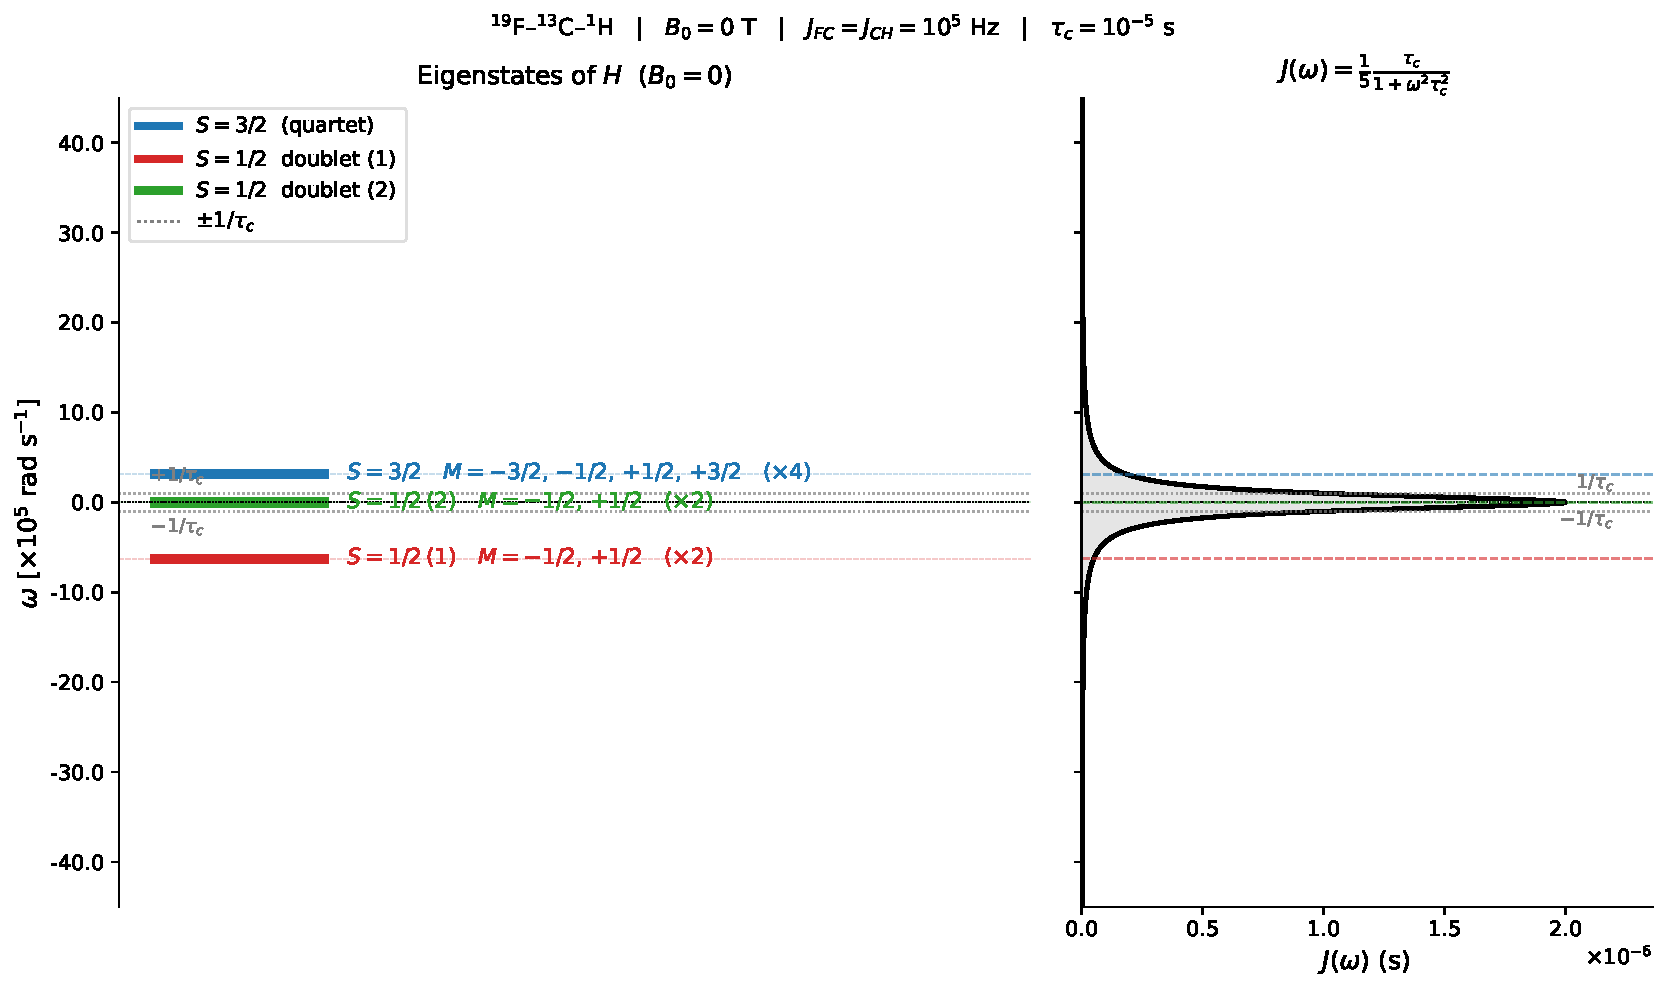
\includegraphics[width=0.8\textwidth]{figs/energy_levels_spectral_density_J1e5}
% Scales image to 80% of text width
 \caption{Comparison between the spectrum of three strongly coupled spins and
the spectral density of the bath, choosing parameters that break density
matrix positivity during evolution, \textit{i.e.} $J\sim1/\tau_{c}$ }
\label{fig:three_spin_st} 
\end{figure}

\begin{figure}
\end{figure}


\section{Linbladian Master equation}

From the previous intuition, we conclude that given the mismatch between
the time-scale of the bath correlation time and the isotropic $J$
couplings in the zero-field limit, density matrix positivity is preserved
and at the same time a Linbladian form of the master equation is warrantied.
For our toy model we have the Hamiltonian
\[
H=\underbrace{\sum_{\langle i,j\rangle}J_{ij}\mathbf{S}_{i}\cdot\mathbf{S}_{j}}_{H_{0}}+H_{DD}(t)
\]
where $H_{DD}(t)$ is the time-modulated dipolar Hamiltonian, which
in an Irreducible Spherical Tensor (IST) basis can be written as
\[
H_{DD}(t)=\sum_{k,m=-2}^{2}D_{k,m}^{(2)}(\Omega(t))\hat{Q}_{k,m}
\]
where 
\[
\hat{Q}_{k,m}=\sum_{i,j}\left(-\frac{\mu_{0}}{4\pi}\frac{\gamma_{i}\gamma_{j}}{r_{ij}^{3}}a_{2,m}^{ij}T_{2,k}^{i,j}\right)
\]
$D_{k,m}^{(2)}(\Omega(t))$ being rank-2 Wigner functions time-modulated
by the function $\Omega(t)$, $T_{2,k}^{i,j}$ being the rank-2 two-body
IST operators for the dipolarly connected spins $i,j$; $a_{2,m}^{ij}$
are orientational factors:

\begin{align}         
a_{2,\pm 2}^{ij} &= \frac{1}{2}\left(a_{x,x}^{ij}-a_{y,y}^{ij} \mp i\left(a_{x,y}^{ij}+a_{y,x}^{ij}\right)\right)\label{eq:alm_start}\\ 
a_{2,\pm 1}^{ij} &= \mp \frac{1}{2}\left(a_{x,z}^{ij}+a_{z,x}^{ij}\mp i \left(a_{y,z}^{ij}+a_{z,y}^{ij}\right)\right)\\     a_{2,0}^{ij} & = \frac{1}{\sqrt{6}}\left(2a_{z,z}^{ij}-\left(a_{x,x}^{ij}+a_{y,y}^{ij}\right)\right)\label{eq:alm_end}. 
\end{align}which are symmetrized linear combinations of elements of the dipolar
tensor $\mathbf{A}$ ($a_{\alpha,\beta}^{ij}=\mathbf{e}_{\alpha}\cdot\mathbf{A}^{ij}\cdot\mathbf{e}_{\beta}$)
\[
H_{DD}=\sum_{i,j}\left(-\frac{\mu_{0}}{4\pi}\frac{\gamma_{i}\gamma_{j}}{r_{ij}^{3}}\right)\mathbf{S}_{i}\cdot\mathbf{A}^{ij}\cdot\mathbf{S}_{j},
\]
and the rest of the prefactors encode the distance-dependent strength
of the dipolar interaction. From de la Pradilla's prescription to
build a Redfield equation in the eigenbasis of $H_{0}$, it suffices
to identify that the bath degrees of freedom are implicitly encoded
in the Wigner functions $D_{k,m}^{(2)}(\Omega(t))$. Ignoring for
the time being Lamb-shifts, we have, for isotropic molecules, that
(\ref{eq:gen_Red})
\begin{align*}
\frac{\gamma_{\alpha,\beta}(\omega)}{2} & =\int_{0}^{\infty}d\tau\langle D_{\alpha}^{(2)}(\tau)D_{\beta}^{(2)}(0)\rangle e^{i\omega\tau}\\
 & =\delta_{\alpha,\beta}J(\omega)
\end{align*}
where we introduce the composite indices $\alpha=(k,m)$ , $\beta=(k',m')$.
From which it follows that 
\begin{align*}
\Gamma_{ij}(\omega) & =\sum_{\alpha\beta}(A_{\alpha})_{i}^{*}\gamma_{\alpha\beta}(\omega)(A_{\beta})_{j}\\
 & =2J(\omega)\sum_{\alpha}(\hat{Q}_{\alpha})_{i}^{*}(\hat{Q}_{\alpha})_{j}
\end{align*}
and $(\hat{Q}_{\alpha})_{j}=\text{Tr}\{\sigma_{j}^{\dagger}\hat{Q}_{\alpha}\}$.
Plugging this in Eq. (\ref{eq:gen_Red}) we get
\begin{align}
\dot{\rho} & =-i[H,\rho]-\frac{1}{4}\sum_{i,j}\left(\Gamma_{ij}(\omega_{j})-\Gamma_{ij}(\omega_{i})\right)[\sigma_{i}^{\dagger}\sigma_{j},\rho]\label{eq:Red_Gamma}\\
 & +\frac{1}{4}\sum_{i,j}\left(\Gamma_{ij}(\omega_{j})+\Gamma_{ij}(\omega_{i})\right)\left(-\{\sigma_{i}^{\dagger}\sigma_{j},\rho\}+2\sigma_{j}\rho\sigma_{i}^{\dagger}\right)\nonumber 
\end{align}
where for completeness in this section $\sigma_{i}=|n_{i}\rangle\langle m_{i}|$,
$|n_{i}\rangle,|m_{i}\rangle$ being eigenstates of $H_{0}$ , and
$\omega_{j}=E_{m_{j}}-E_{n_{j}}$ is the energy for transition $j$.
One inmediate question here, to understand the selection rules for
transitions between $H_{0}$ eigenstates, is how the symmetry-adapted
observables $\hat{Q}_{k,m}$ act on the eigenstates of the isotropic
Hamiltonian $H_{0}$. More precisely, for 
\[
\hat{Q}_{k,m}|J,M\rangle=\sum_{K,L}c_{KL}^{(k,m)}|K,L\rangle
\]
the question is to find which amplitudes$c_{KL}^{(k,m)}$ are not
vanishing.

\subsection{Fermi's Golden Rule}

Getting some intuition on what are the dominant transition rates across
populations in the dynamics in the low-field limit. Taking as our
starting point the time domain formulation of FGR:
\begin{align*}
k_{i\rightarrow f}(\omega) & =\int_{0}^{\infty}d\tau\langle V_{fi}(t)V_{fi}^{\dagger}(0)\rangle
\end{align*}
where we make the indentification $V\rightarrow H_{DD}(t)=\sum_{k,m}D_{k,m}(t)Q_{k,m}$.
To get 
\[
k_{i\rightarrow f}=\sum_{k,m}\sum_{k',m'}\int_{0}^{\infty}d\tau e^{i\omega_{fi}\tau}\langle D_{k,m}(\tau)D_{k',m'}(0)\rangle\langle f|Q_{k,m}|i\rangle\langle i|Q_{k',m'}|f\rangle
\]
where we considered $|i\rangle,|f\rangle$ being eigenstates of the
spin Hamiltonian, $\omega_{fi}=\omega_{f}-\omega_{i}$ where $\omega_{j}$
is the eigenfrequency of the $j$th eigenstate. For isotropic tumbling
we have
\[
k_{i\rightarrow f}(\omega)=J(\omega_{fi})\sum_{k,m}|\langle f|Q_{k,m}|i\rangle|^{2}
\]
Table~\ref{tab:fgr_rates} lists the five largest rates computed
numerically for$\tau_{c}=10^{-5}$ s and$B_{0}=0$, using the physical
geometry and couplings of the$^{19}$F--$^{13}$C--$^{1}$H system.

\begin{table}[h!]
\centering%
\begin{tabular}{cccrr}
\hline 
Rank & Initial$|i\rangle$ & Final$|f\rangle$ & $\omega_{fi}/(2\pi)$ {[}Hz{]} & $k/(2\pi)$ {[}Hz{]}\tabularnewline
\hline 
1 & $|1/2_{\beta},-1/2\rangle$ & $|3/2,+3/2\rangle$ & $+7.94$ & $1603$\tabularnewline
2 & $|3/2,+3/2\rangle$ & $|1/2_{\beta},-1/2\rangle$ & $-7.94$ & $1603$\tabularnewline
3 & $|3/2,-3/2\rangle$ & $|1/2_{\beta},+1/2\rangle$ & $-7.94$ & $1603$\tabularnewline
4 & $|1/2_{\beta},+1/2\rangle$ & $|3/2,-3/2\rangle$ & $+7.94$ & $1603$\tabularnewline
5 & $|3/2,+1/2\rangle$ & $|1/2_{\beta},-1/2\rangle$ & $-7.94$ & $1202$\tabularnewline
 &  &  &  & \tabularnewline
\hline 
\end{tabular}\caption{Top-5 Fermi's Golden Rule population-transfer rates$k_{i\to f}=J(\omega_{fi})\sum_{k,m}|\langle f|Q_{k,m}|i\rangle|^{2}$
between eigenstates of$H_{0}$, computed for$\tau_{c}=10^{-5}$ s,$B_{0}=0$.
States$|1/2_{\beta},M\rangle$ are the higher-energy$S=1/2$ doublet;$|3/2,M\rangle$
are the quartet states. Rates 1--4 are the two time-reversal pairs
at the$S=3/2\leftrightarrow S=1/2_{\beta}$ gap$|\omega_{fi}|/(2\pi)\approx7.94$
Hz; rate 5 involves a different$\Delta M$ channel at the same gap.
All transitions are forbidden within the doublet sector, consistent
with the triangle rule.}
\label{tab:fgr_rates}
\end{table}

Table~\ref{tab:fgr_uuu} restricts the view to the initial state$|3/2,+3/2\rangle=|\!\uparrow\uparrow\uparrow\rangle$,
exposing the outflow channels that govern the early-time dynamics.

\begin{table}[h!]
\centering%
\begin{tabular}{ccrr}
\hline 
Rank & Final$|f\rangle$ & $\omega_{fi}/(2\pi)$ {[}Hz{]} & $k/(2\pi)$ {[}Hz{]}\tabularnewline
\hline 
1 & $|1/2_{\beta},-1/2\rangle$ & $-7.94$ & $1603$\tabularnewline
2 & $|3/2,+1/2\rangle$ & $0$ & $1077$\tabularnewline
3 & $|3/2,-1/2\rangle$ & $0$ & $1077$\tabularnewline
4 & $|1/2_{\beta},+1/2\rangle$ & $-7.94$ & $401$\tabularnewline
5 & $|1/2_{\alpha},-1/2\rangle$ & $-246.27$ & $1.29$\tabularnewline
 &  &  & \tabularnewline
\hline 
\end{tabular}\caption{Top-5 FGR transfer rates out of$|3/2,+3/2\rangle=|\!\uparrow\uparrow\uparrow\rangle$,
for$\tau_{c}=10^{-5}$ s,$B_{0}=0$. Ranks 2--3 are intra-quartet
($\omega_{fi}=0$, driven by$\Delta M=-1$ and$\Delta M=-2$ components
of$Q_{k,m}$); ranks 1 and 4 cross into$S=1/2_{\beta}$ at the 7.94~Hz
gap. Rank 5, reaching the lower-energy$S=1/2_{\alpha}$ doublet at
a 246~Hz gap, is three orders of magnitude slower because the$\alpha$
doublet has predominantly pair-singlet character and therefore a small
reduced matrix element. No intra-doublet transitions appear, consistent
with the triangle-rule selection rules.}
\label{tab:fgr_uuu}
\end{table}


\subsection{Relaxation matrix verification}

Reproduction of the reference Redfield dynamics through Spinach package
remains an elusive task. Comparison between the Redfield relaxation
matrix (in the Liouville Pauli basis) and the Linbladian one flags
an almost two-order-of-magnitude mismatch between 3 diagonal matrix
elements. Closer inspection of this mismatch might reveal the root
of the issues. 

At its core, in terms of Hamiltonian and relaxation super-operators
we have 
\[
\partial_{t}\rho=-i\mathcal{H}_{0}\rho+\mathcal{R}\rho
\]
where 
\[
\mathcal{R}=-\sum_{\alpha,\beta}\int_{0}^{\infty}d\tau g_{\alpha,\beta}(\tau)\mathcal{Q}_{\alpha}e^{-i\mathcal{H}_{0}\tau}\mathcal{Q}_{\beta}^{\dagger}e^{i\mathcal{H}_{0}\tau}
\]
and we used the composite indices $\alpha=k,m$. Decomposing the super-operators
in terms of the $\mathcal{H}_{0}$ eigenbasis we have 
\[
\mathcal{R}=-\sum_{\alpha,\beta}\sum_{i,j}\int_{0}^{\infty}d\tau g_{\alpha,\beta}(\tau)e^{-i\omega_{j}\tau}c_{i}^{\alpha}c_{j}^{\beta*}\mathcal{P}_{i}\mathcal{P}_{j}^{\dagger}
\]
where the composite indices $i,j$ label transition operators of the
form $|n_{j}\rangle\langle m_{j}|$ with a corresponding transition
frequency $\omega_{j}=\omega_{n_{j}}-\omega_{m_{j}}$, $H_{0}|n_{j}\rangle=\omega_{n_{j}}|n_{j}\rangle$,
and $c_{i}^{\alpha}=\text{Tr}\{\sigma_{i}^{\dagger}\mathcal{Q}_{\alpha}\}$.
To make the connection with the Redfield form above we identify $\Gamma_{ij}(\omega)=\sum_{\alpha,\beta}\int_{0}^{\infty}d\tau g_{\alpha,\beta}(\tau)e^{-i\omega\tau}c_{i}^{\alpha}c_{j}^{\beta*}$,
such that
\begin{align*}
\mathcal{R}[\rho] & =-\sum_{i,j}\Gamma_{ij}(\omega_{j})[\sigma_{i},[\sigma_{j}^{\dagger},\rho]]\\
 & =-\sum_{i,j}\Gamma_{ij}(\omega_{j})[\sigma_{i}^{\dagger},[\sigma_{j},\rho]]\\
 & =-\frac{1}{2}\sum_{i,j}\Gamma_{ij}(\omega_{j})[\sigma_{i}^{\dagger},[\sigma_{j},\rho]]-\frac{1}{2}\sum_{i,j}\Gamma_{ij}(\omega_{i})[\sigma_{j},[\sigma_{i}^{\dagger},\rho]]\\
 & =-\frac{1}{2}\sum_{i,j}\Gamma_{ij}(\omega_{j})\left(\sigma_{i}^{\dagger}\sigma_{j}\rho-\sigma_{i}^{\dagger}\rho\sigma_{j}-\sigma_{j}\rho\sigma_{i}^{\dagger}+\rho\sigma_{j}\sigma_{i}^{\dagger}\right)\\
 & -\frac{1}{2}\sum_{i,j}\Gamma_{ij}(\omega_{i})\left(\sigma_{j}\sigma_{i}^{\dagger}\rho-\sigma_{j}\rho\sigma_{i}^{\dagger}-\sigma_{i}^{\dagger}\rho\sigma_{j}+\rho\sigma_{i}^{\dagger}\sigma_{j}\right)\\
 & =-\sum_{ij}\frac{\Gamma_{ij}(\omega_{i})+\Gamma_{ij}(\omega_{j})}{2}\{\sigma_{i}^{\dagger}\sigma_{j},\rho\}-\sum_{ij}(\Gamma_{ij}(\omega_{i})+\Gamma_{ij}(\omega_{j}))\sigma_{i}^{\dagger}\rho\sigma_{j}\\
 & +\sum_{i,j}\frac{\Gamma_{ij}(\omega_{i})-\Gamma_{ij}(\omega_{j})}{2}[\sigma_{i}^{\dagger}\sigma_{j},\rho]
\end{align*}
\linebreak{}


\subsection{Core tool: Wigner--Eckart theorem}

The key structural observation is that $T_{2,k}^{i,j}$, and therefore$\hat{Q}_{k,m}$
(for fixed $m$, as a function of$k$), is a\emph{ rank-2 irreducible
spherical tensor operator under global rotations of all spins.} This
follows because$T_{2,k}^{i,j}$ is a bilinear combination of single-spin
operators that transforms as$D^{(2)}$ under$e^{i\theta\mathbf{n}\cdot\mathbf{J}_{\mathrm{tot}}}$;
the fact that it only has support on the pair$(i,j)$ is irrelevant
for its transformation properties under global rotations. Since$H_{0}$
is rotationally invariant, its eigenstates$|J,M\rangle$ carry good
total angular momentum, and the Wigner--Eckart theorem gives
\begin{equation}
\langle K,L,\nu'|\hat{Q}_{k,m}|J,M,\nu\rangle=\langle J,M;\,2,k\,|\,K,L\rangle\,\langle K,\nu'\|\hat{Q}_{m}\|J,\nu\rangle,\label{eq:WE}
\end{equation}
where$\nu,\nu'$ are multiplicity labels distinguishing degenerate$J$
sectors (relevant for$N\geq3$ spins), and$\langle K,\nu'\|\hat{Q}_{m}\|J,\nu\rangle$
is the reduced matrix element, which carries all the dynamics but
is independent of$M$ and$L$. The Clebsch--Gordan coefficient alone
imposes two\emph{ kinematic} selection rules:
\begin{itemize}
\item $\Delta M=k$: the component index$k\in\{-2,-1,0,+1,+2\}$ sets the
change in the magnetic quantum number.
\item Triangle rule:$|J-2|\leq K\leq J+2$. Combined with the physical constraint$K\leq N/2$,
this restricts which$J$-sectors can be connected.
\end{itemize}

\subsection{Selection rules: two-spin and three-spin cases}

\textbf{Two spins} ($J\in\{0,1\}$). For the singlet$|J=0\rangle$:
the triangle rule requires$|0-2|=2\leq K$, but$K\leq1$ for two spins-$\tfrac{1}{2}$.
No$K$ satisfies both constraints simultaneously, so all Clebsch--Gordan
coefficients$\langle0,0;\,2,k\,|\,K,L\rangle$ vanish identically
for any$k$. The singlet is dark for\emph{ all} components$k$ and\emph{
all} spatial indices$m$---a purely kinematic result requiring no
explicit matrix computation. For the triplet$|J=1\rangle$: the intersection
of$\{|1-2|,\ldots,3\}=\{1,2,3\}$ with$K\leq1$ gives$K=1$ only,
so the triplet maps only into itself.

\textbf{Three spins} ($J\in\{1/2,3/2\}$, with the doublet$J=1/2$
having multiplicity 2).
\begin{itemize}
\item From$|J=1/2\rangle$: triangle rule gives$K\in\{3/2,5/2\}$; with$K\leq3/2$
only$K=3/2$ survives.\emph{ Doublet$\to$ quartet only; doublet$\to$
doublet transitions are forbidden by the triangle rule.}
\item From$|J=3/2\rangle$: triangle rule gives$K\in\{1/2,3/2\}$. The quartet
can scatter into both doublets and remain in the quartet.
\end{itemize}
This is the quantitative underpinning of the cross-manifold leakage
discussed in Section~6.3: the relaxation superoperator opens quartet$\leftrightarrow$
doublet channels precisely because the triangle rule permits it, whereas
within the doublet sector the triangle rule strictly forbids any transition.

\subsection{Transition amplitudes: reduced matrix elements via 6j symbols}

The selection rules above are kinematic. The actual transition amplitudes
are encoded in the reduced matrix element$\langle K,\nu'\|\hat{Q}_{m}\|J,\nu\rangle$.
For a pair operator$T_{2,k}^{(12)}$ acting only on spins 1 and 2,
with spin 3 as a spectator, the standard recoupling identity gives
\begin{equation}
\langle J',S_{12}'\|T_{2}^{(12)}\|J,S_{12}\rangle=(-1)^{S_{12}'+I_{3}+J+2}\sqrt{(2J'+1)(2J+1)}\begin{Bmatrix}S_{12} & S_{12}' & 2\\
J' & J & I_{3}
\end{Bmatrix}\langle S_{12}'\|T_{2}^{(12)}\|S_{12}\rangle,\label{eq:6j}
\end{equation}
where$I_{3}=1/2$ is the spectator spin, the curly bracket is a Wigner
6j symbol, and$\langle S_{12}'\|T_{2}^{(12)}\|S_{12}\rangle$ is the
two-spin reduced matrix element, which vanishes for$S_{12}=0$ (the
pair-singlet dark state, Eq.~\eqref{eq:dark}). For$N=3$ spins,
each of the three pairs contributes a term of the form\eqref{eq:6j}
(with the appropriate spectator spin), and the total reduced matrix
element is their sum. Whether contributions add constructively or
cancel depends on the molecular geometry (which pairs are dipolar-coupled)
and can be evaluated once a consistent$S_{12}$-labelled basis is
fixed.

\subsection{Change of jump operator basis}

Eq.~(\ref{eq:Red_Gamma}) can be rendered in the IST basis by projecting the transition operators $\sigma_{j}$ onto the normalised IST operators $\hat{p}_{\delta}$
\begin{align}
\dot{\rho} & =-i[H,\rho]-\sum_{i,j}\Gamma_{ij}^{(-)}[\sigma_{i}^{\dagger}\sigma_{j},\rho]+\sum_{i,j}\Gamma_{ij}^{(+)}\left(-\{\sigma_{i}^{\dagger}\sigma_{j},\rho\}+2\sigma_{j}\rho\sigma_{i}^{\dagger}\right)\nonumber\\
 & =-i[H,\rho]-\sum_{ij}\sum_{\mu,\delta}\Gamma_{ij}^{(-)}c_{i,\mu}^{*}c_{j,\delta}[\hat{p}_{\mu}^{\dagger}\hat{p}_{\delta},\rho]\nonumber\\
 & \quad+\sum_{i,j}\sum_{\mu,\delta}\Gamma_{ij}^{(+)}c_{i,\mu}^{*}c_{j,\delta}\left(-\{\hat{p}_{\mu}^{\dagger}\hat{p}_{\delta},\rho\}+2\hat{p}_{\delta}\rho\hat{p}_{\mu}^{\dagger}\right)\nonumber\\
 & =-i[H,\rho]-\sum_{\mu,\delta}\Delta_{\mu,\delta}^{(-)}[\hat{p}_{\mu}^{\dagger}\hat{p}_{\delta},\rho]+\sum_{\mu,\delta}\Delta_{\mu,\delta}^{(+)}\left(-\{\hat{p}_{\mu}^{\dagger}\hat{p}_{\delta},\rho\}+2\hat{p}_{\delta}\rho\hat{p}_{\mu}^{\dagger}\right)\label{eq:chg_bas}
\end{align}
where $c_{j,\delta}=\mathrm{Tr}\{\hat{p}_{\delta}^{\dagger}\sigma_{j}\}$ and
\begin{align*}
\Delta_{\mu,\delta}^{(-)} & =\sum_{ij}\Gamma_{ij}^{(-)}c_{i,\mu}^{*}c_{j,\delta}\\
\Delta_{\mu,\delta}^{(+)} & =\sum_{i,j}\Gamma_{ij}^{(+)}c_{i,\mu}^{*}c_{j,\delta}
\end{align*}
What is the ``boddyness\textquotedblright{} of the predominant channels $(\delta,\mu)$? Can we leverage the symmetry of the transition operators $\sigma_{i}=|S_{1}^{(i)},M_{1}^{(i)}\rangle\langle S_{2}^{(i)},M_{2}^{(i)}|$ to derive selection rules for non-vanishing inner products $\langle\langle T_{m}^{(l)}|\sigma_{i}\rangle\rangle$ in Liouville space, where $T_{m}^{(l)}$ is a many-body tensor of rank $l$?

Following the intuition that spins decohere on a timescale $\tau_{c}\ll1/J_{H}$, $J_{H}$ being a characteristic Heisenberg energy scale, the Lindblad operators are expected to preserve the ``two-bodyness\textquotedblright{} of dipolar interactions. The master equation is therefore projected into the two-spin rank-2 IST basis $T_{ij}^{(l=2,m)}$ (indices $i,j$ label a spin pair), corresponding to the change of basis in Eq.~(\ref{eq:chg_bas}) with $\{\hat{p}_{i}\}=\{T_{ij}^{(l=2,m)}\}$.

The five dominant canonical Lindblad operators $\hat{L}_{k}=\sum_{\delta}U_{\delta k}^{*}\hat{p}_{\delta}$ are listed in Table~\ref{tab:dom5}, decomposed into the normalised two-spin rank-2 IST basis $\{\hat{p}_{\delta}\}$ (unit Hilbert--Schmidt norm).

\begin{table}[h]
\centering
\medskip
\begin{tabular}{lrrrrr}
\hline\hline
(a)~$^{19}\mathrm{F}$--$^{13}\mathrm{C}$ & $k=-2$ & $k=-1$ & $k=0$ & $k=+1$ & $k=+2$ \\
\hline
$\hat{L}_{1}$ & $+0.9971$ & $+0.0000$ & $+0.0000$ & $+0.0000$ & $+0.0000$ \\
$\hat{L}_{2}$ & $-0.0000$ & $+0.0914$ & $+0.0119$ & $-0.1234$ & $+0.9852$ \\
$\hat{L}_{3}$ & $+0.0000$ & $-0.8828$ & $-0.2426$ & $+0.3724$ & $+0.1315$ \\
$\hat{L}_{4}$ & $-0.0000$ & $+0.1146$ & $-0.9353$ & $-0.3236$ & $-0.0398$ \\
$\hat{L}_{5}$ & $+0.0000$ & $-0.4397$ & $+0.2458$ & $-0.8577$ & $-0.0697$ \\
\hline
\end{tabular}

\medskip
\begin{tabular}{lrrrrr}
\hline\hline
(b)~$^{19}\mathrm{F}$--$^{1}\mathrm{H}$ & $k=-2$ & $k=-1$ & $k=0$ & $k=+1$ & $k=+2$ \\
\hline
$\hat{L}_{1}$ & $+0.0708$ & $+0.0000$ & $+0.0000$ & $+0.0000$ & $+0.0000$ \\
$\hat{L}_{2}$ & $+0.0000$ & $+0.0065$ & $+0.0008$ & $-0.0088$ & $+0.0700$ \\
$\hat{L}_{3}$ & $+0.0000$ & $-0.0627$ & $-0.0172$ & $+0.0265$ & $+0.0093$ \\
$\hat{L}_{4}$ & $+0.0000$ & $+0.0081$ & $-0.0665$ & $-0.0230$ & $-0.0028$ \\
$\hat{L}_{5}$ & $-0.0000$ & $-0.0312$ & $+0.0175$ & $-0.0609$ & $-0.0050$ \\
\hline
\end{tabular}

\medskip
\begin{tabular}{lrrrrr}
\hline\hline
(c)~$^{13}\mathrm{C}$--$^{1}\mathrm{H}$ & $k=-2$ & $k=-1$ & $k=0$ & $k=+1$ & $k=+2$ \\
\hline
$\hat{L}_{1}$ & $+0.0270$ & $+0.0000$ & $+0.0000$ & $+0.0000$ & $+0.0000$ \\
$\hat{L}_{2}$ & $+0.0000$ & $+0.0025$ & $+0.0003$ & $-0.0033$ & $+0.0267$ \\
$\hat{L}_{3}$ & $-0.0000$ & $-0.0239$ & $-0.0066$ & $+0.0101$ & $+0.0036$ \\
$\hat{L}_{4}$ & $-0.0000$ & $+0.0031$ & $-0.0254$ & $-0.0088$ & $-0.0011$ \\
$\hat{L}_{5}$ & $+0.0000$ & $-0.0119$ & $+0.0067$ & $-0.0233$ & $-0.0019$ \\
\hline
\end{tabular}

\caption{\label{tab:dom5}Decomposition of the five dominant canonical Lindblad operators $\hat{L}_{k}$ in the normalised two-spin rank-2 IST basis $\hat{p}_{\delta}=T_{\delta}^{(2,k)}/\|T_{\delta}^{(2,k)}\|_{\mathrm{HS}}$. Sub-tables (a), (b), (c) list coefficients $U_{\delta k}^{*}$ for the $^{19}\mathrm{F}$--$^{13}\mathrm{C}$, $^{19}\mathrm{F}$--$^{1}\mathrm{H}$, and $^{13}\mathrm{C}$--$^{1}\mathrm{H}$ pairs respectively. Dephasing rate: $2d_{k}/(2\pi)=10616\,\mathrm{Hz}$.}
\end{table}


\section{Universal Linbladian formalism}
Here it is useful to define tensor operators associated to the rotation group

        \begin{align}
            H_1(t) &= \sum_{\mu m l} \Phi^{(l,m)}_\mu(t) T_\mu^{(l,m)}
        \end{align}
Under rotational diffusion we have 
        \begin{align}
    \overline{\left(\Phi^{(l,m)}_\mu(t)\right)^\dagger \Phi^{(l',m')}_\nu(t')} &=\frac{1}{2l+1} \delta^{ll'}\delta^{mm
            '}\mathcal{N}^{(l,m)}_{\mu \nu} \exp(-|t-t'|/\tau_l)
        \end{align}

where $1/\tau_l=l(l+1)D_r$ where $D_r$ is the rotational diffusion coefficient.

Intuitively, the matrix $\mathcal{N}^{(l,m)}$ encodes the \textit{noise power covariance} generated by the \textit{collectively fluctuating} dipolar interactions. For each $m$, we diagonalize this matrix $\mathcal{N}$, 

    \begin{align}
        \left(U^{(l,m)}\right)^\dagger \mathcal{N}^{(l,m)} U^{(l,m)} =  \text{diag}\left(\left\lbrace \left(\gamma^{(l,m)}_{\alpha}\right)^2\right\rbrace_\alpha \right) \
    \end{align}
    
    The relevant spectral function will then be 

    \begin{align}
        S^{(l,m)}_{\alpha\alpha}(\omega) &= \frac{\left(\gamma^{(l,m)}_{\alpha}\right)^2}{2l+1} \frac{2/\tau_l}{\omega^2+(1/\tau_l)^2} 
    \end{align}
    For the particular case where $H_{1}(t)$ corresponds to dipolar interactions, it follows that 
    \begin{equation}
    \mathcal{N}^{l,m}_{\mu\nu} = \left(\frac{\mu_{0}}{4\pi}\right)^{2}\left(\frac{\gamma_{\mu_{i}}\gamma_{\mu_{j}}}{r^{3}_{\mu}}\right)\left(\frac{\gamma_{\nu_{i}}\gamma_{\nu_{j}}}{r^{3}_{\nu}}\right)a^{(\mu)}_{l,m}a^{(\nu)}_{l,m}
    \end{equation}
    where $\mu,\nu$ are composite indices that label spin pairs, the orientational factors $a^{(\mu)}_{l,m}$ are defined in \ref{eq:alm_end}, where we note that they vanish unless $l=2$, and $r_{\mu} = |r_{\mu_{i}}-r_{\mu_{j}}|$ is the distance between spin pairs $\mu_{i},\mu_{j}$. \\
    Skipping the details of derivation, and ignoring operator dressing due to the Heisenberg couplings, it turns out that the jump operators that enter into a Linbladian master equation description of dipolar coupled spins is 

\begin{equation}
L_\alpha^{(2,m)} &\equiv \sqrt{\frac{\left(\gamma_\alpha^{(l,m)}\right)^2\tau_c}{5}} \sum_\mu \phi_\alpha^{(m)}(\mu) T^{(2,m)}_\mu
\end{equation}    
where $\phi^{m}_{\alpha}(\mu)$ correspond to the coefficients of the $\alpha$th eigenvector of $\mathcal{N}^{2,m}$, and $\tau_c$ as defined above, is the correlation time of the solvent.
    



\section{Gemcitabine parameters}

Spin-system parameters for Gemcitabine from a Gaussian quantum-chemistry
calculation. The 10 nuclei are ordered as$(F_{0},F_{1},H_{0},H_{1},H_{2},H_{3},H_{4},H_{5},H_{6},C_{0})$,
comprising two$^{19}\mathrm{F}$, seven$^{1}\mathrm{H}$, and one$^{13}\mathrm{C}$.

\subsection{J-coupling matrix (Hz)}

Scalar couplings$J_{ij}$ in Hz, upper triangular; dots denote symmetric
lower entries.
\[
J={\scriptscriptstyle \begin{pmatrix}0 & 175.91 & 0.00 & 0.11 & 0.05 & 6.66 & -0.32 & 0.05 & 11.59 & -226.85\\
\cdot & 0 & 0.09 & -0.20 & 0.28 & 5.91 & 0.08 & -0.09 & 0.48 & -203.41\\
\cdot & \cdot & 0 & -3.66 & 0.73 & -0.14 & -0.10 & -0.11 & 0.18 & -0.13\\
\cdot & \cdot & \cdot & 0 & 2.88 & -0.12 & -0.10 & -0.10 & 0.38 & -0.10\\
\cdot & \cdot & \cdot & \cdot & 0 & 0.22 & 0.02 & -0.09 & 2.12 & 0.31\\
\cdot & \cdot & \cdot & \cdot & \cdot & 0 & 0.38 & -0.07 & -0.37 & -0.65\\
\cdot & \cdot & \cdot & \cdot & \cdot & \cdot & 0 & 2.67 & -0.15 & 0.02\\
\cdot & \cdot & \cdot & \cdot & \cdot & \cdot & \cdot & 0 & -0.14 & -0.08\\
\cdot & \cdot & \cdot & \cdot & \cdot & \cdot & \cdot & \cdot & 0 & -2.68\\
\cdot & \cdot & \cdot & \cdot & \cdot & \cdot & \cdot & \cdot & \cdot & 0
\end{pmatrix}}
\]


\subsection{Nuclear coordinates}

\begin{tabular}{crrr}
\hline 
Nucleus & $x$ (�) & $y$ (�) & $z$ (�)\tabularnewline
\hline 
$F_{0}$ & 0.1666 & \textminus 1.2783 & \textminus 1.3875\tabularnewline
$F_{1}$ & 0.9661 & \textminus 2.5748 & 0.3352\tabularnewline
$H_{0}$ & 4.2344 & 1.2314 & \textminus 0.5006\tabularnewline
$H_{1}$ & 2.7307 & 1.8998 & \textminus 1.1779\tabularnewline
$H_{2}$ & 2.8928 & 0.2529 & 1.3947\tabularnewline
$H_{3}$ & 0.4474 & \textminus 0.6659 & 1.8321\tabularnewline
$H_{4}$ & \textminus 1.7462 & \textminus 0.8907 & 2.3837\tabularnewline
$H_{5}$ & \textminus 4.1117 & \textminus 0.4940 & 1.8959\tabularnewline
$H_{6}$ & 2.4649 & \textminus 0.4748 & \textminus 1.5086\tabularnewline
$C_{0}$ & 0.9133 & \textminus 1.2851 & \textminus 0.2046\tabularnewline
\hline 
\end{tabular}

\subsection{Zeeman (chemical shielding) matrices (ppm)}

\[
\boldsymbol{\sigma}(F_{0})=\begin{pmatrix}-130.0601 & -14.9649 & -63.1405\\
-14.9649 & -215.3146 & 25.9348\\
-63.1405 & 25.9348 & -160.2068
\end{pmatrix}
\]

\[
\boldsymbol{\sigma}(F_{1})=\begin{pmatrix}-157.2094 & -12.7347 & -67.3755\\
-12.7347 & -235.8144 & 5.7085\\
-67.3755 & 5.7085 & -228.8689
\end{pmatrix}
\]

\[
\boldsymbol{\sigma}(H_{0})=\begin{pmatrix}2.2651 & -0.6354 & 2.4859\\
-0.6354 & 2.7073 & -2.7546\\
2.4859 & -2.7546 & 6.9013
\end{pmatrix}
\]

\[
\boldsymbol{\sigma}(H_{1})=\begin{pmatrix}7.0348 & -2.4557 & -1.2496\\
-2.4557 & 3.6480 & -0.3257\\
-1.2496 & -0.3257 & 1.9779
\end{pmatrix}
\]

\[
\boldsymbol{\sigma}(H_{2})=\begin{pmatrix}1.5527 & 0.6046 & -2.3124\\
0.6046 & 5.3322 & 0.1728\\
-2.3124 & 0.1728 & 4.7300
\end{pmatrix}
\]

\[
\boldsymbol{\sigma}(H_{3})=\begin{pmatrix}4.3528 & -1.0174 & 1.5080\\
-1.0174 & 5.8782 & 1.7827\\
1.5080 & 1.7827 & 3.5154
\end{pmatrix}
\]

\[
\boldsymbol{\sigma}(H_{4})=\begin{pmatrix}3.1215 & 0.1121 & 1.7281\\
0.1121 & 9.5089 & 0.5658\\
1.7281 & 0.5658 & 7.4617
\end{pmatrix}
\]

\[
\boldsymbol{\sigma}(H_{5})=\begin{pmatrix}2.5152 & 0.8210 & -0.8704\\
0.8210 & 6.6786 & 1.2727\\
-0.8704 & 1.2727 & 4.7920
\end{pmatrix}
\]

\[
\boldsymbol{\sigma}(H_{6})=\begin{pmatrix}4.4701 & 0.6055 & 0.2616\\
0.6055 & 4.4715 & 1.0493\\
0.2616 & 1.0493 & 2.7238
\end{pmatrix}
\]

\[
\boldsymbol{\sigma}(C_{0})=\begin{pmatrix}241.3681 & -1.4291 & -6.1424\\
-1.4291 & 245.7345 & 3.0563\\
-6.1424 & 3.0563 & 250.0215
\end{pmatrix}
\]




\end{document}
